\documentclass[
    a4paper,
    12pt,
    addpoints,
    % answers
]{exam}
\usepackage[utf8]{inputenc}
\usepackage[T1]{fontenc}
\usepackage[lmargin=3cm,rmargin=2cm,tmargin=2cm,bmargin=2cm]{geometry}
\usepackage[brazil]{babel}

\usepackage{graphicx}
\usepackage{xcolor}
\usepackage[]{hyperref}

\pagestyle{headandfoot}
\firstpageheadrule
\firstpageheader{Nightwind \\ Professor}{\large \sffamily Primeiro Trabalho \\ Disciplina: \LaTeX}{25 de março de 2021}

\firstpagefootrule
\firstpagefooter{\bfseries \sffamily Nightwind}{}{\itshape \ttfamily Bom Trabalho!}

\runningheadrule
\runningheader{Primeiro Trabalho}{}{\makebox[5cm]{Matrícula:\enspace\hrulefill}}

\runningfooter{Nightwind}{Bom Trabalho!}{Página \thepage \, de \numpages.}
\runningfootrule

% \pointname{\%}
\pointpoints{ponto}{pontos}
\bonuspointpoints{ponto (bônus)}{pontos (bônus)}
% \boxedpoints
% \bracketedpoints

% \pointsinmargin
% \marginpointname{\%}


\renewcommand{\solutiontitle}{\noindent\textbf{Solução:}\par\noindent}
\colorfillwithlines
\definecolor{FillWithLinesColor}{gray}{0.8}
\setlength{\gridsize}{5mm}
\colorgrids
\definecolor{GridColor}{rgb}{0.8,0.85,1}
\colorfillwithdottedlines
\definecolor{FillWithDottedLinesColor}{gray}{0.8}


\hqword{Questão}
\hpgword{Página}
\hpword{Valor}
\hsword{Pontos}
\htword{Total} 


\begin{document}

\begin{center}
    \fbox{\fbox{\parbox{0.5\textwidth}{
        Para este trabalho é permitido:
        \begin{itemize}
            \item usar calculadora;
            \item entregar a prova a lápis;
            \item consultar os materiais; e,
            \item consultar os colegas.
        \end{itemize}
    }}}
\end{center}
    \makebox[\textwidth]{Nome e matrícula:\enspace\hrulefill}

\begin{center}
    \gradetable[h][questions]
\end{center}

    \begin{questions}
        \question[2] Questão 1: 
        \begin{parts}
            \part[1] Pergunta a da \autoref{question@1}:
            \begin{solutionorbox}[1in]
                A solução é esta.
            \end{solutionorbox}
            \part[1] Pergunta b da \autoref{question@1}
            \begin{solutionordottedlines}[1in]
                A solução é esta.
            \end{solutionordottedlines}
        \end{parts}

        \question[5] Qual a tabela verdade 
        \begin{solutionorgrid}[2.5cm]
            \begin{tabular}{|l|l|l|}
                \hline 
                A & B & S \\ \hline
                0 & 0 & 0 \\ \hline
                0 & 1 & 0 \\ \hline
                1 & 0 & 0 \\ \hline
                1 & 1 & 1 \\ \hline
            \end{tabular}
        \end{solutionorgrid}

        \question[4] Descreva o funcionamento de 
        \begin{figure}[h]
            \centering
            % \caption{}
            % \label{}
            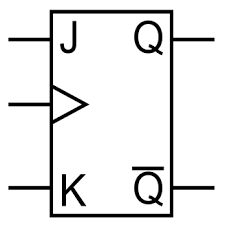
\includegraphics[width=2cm]{ffjk.png}
        \end{figure}
        \begin{solutionorlines}[1in]
            Funciona assim...
        \end{solutionorlines}
        \question Preenchas as lacunas: 
        \begin{parts}
            \part Com relação ao uso de máscaras:
            \begin{subparts}
                \subpart[4] O uso de \fillin[máscaras][3cm] é \fillin[obrigatório][2.5cm] porque \fillin[protege][2cm] todos ao redor.
                \subpart Marque (V) para verdadeiro e (F) para falso.
                \begin{subsubparts}
                    \subsubpart[3] (\fillin[F][0.5cm]) primeira sentença.
                    \subsubpart[3] (\fillin[V][0.5cm]) segunda sentença.
                    \subsubpart[3] (\fillin[F][0.5cm]) terceira sentença.
                    \subsubpart[3] (\fillin[V][0.5cm]) quarta sentença.
                    \subsubpart[3] (\fillin[F][0.5cm]) quinta sentença.
                    \subsubpart[3] (\fillin[V][0.5cm]) sexta sentença.
                    \subsubpart[3] (\fillin[F][0.5cm]) sétima sentença. 
                \end{subsubparts}
            \end{subparts}
        \end{parts}

        \question Questões de múltipla escolha:
        \begin{parts}
            \part[3] Onde vende água?
            \begin{choices}
                \choice Farmácia.
                \choice Mercado.
                \CorrectChoice Mercearia.
                \choice Restaurante.
            \end{choices}

            \part[3] Onde vende água?

            \begin{oneparchoices}
                \choice Farmácia.
                \choice Mercado.
                \CorrectChoice Mercearia.
                \choice Restaurante.
            \end{oneparchoices}

        \end{parts}
    \end{questions}
\end{document}